\pgfplotstablegetelem{\thepart}{[index]\columnIndex}\of{\cronograma}
\part{\pgfplotsretval}
\label{part:\thepart}
\frame{\partpage}


\begin{frame}[t]{Programação Orientada a Objetos}
	
	\fontsize{14pt}{15}\selectfont{
		
		...continuando a partir da aula passada sobre \gls{poo}.
		
	}\par
	\vspace{1em}
	
	
\end{frame}




\begin{frame}[t]{Programação Orientada a Objetos}
	
	\fontsize{14pt}{15}\selectfont{
		
		...relembrando a última aula:
				
	}\par
	\vspace{1em}
	
	\fontsize{12pt}{15}\selectfont{
		\begin{itemize}%[<+->] 
			
			\item Na terminologia Python a classe original é chamada de Classe Base, Classe Mãe ou Superclasse (Base, Parent ou Super Class) enquanto que a nova é chamada de Sub Classe ou Classe Filha (Sub ou Child Class).
			
			\item A subclasse pode especializar a classe principal ou mesmo estendê-la com novos métodos e atributos.
			
		\end{itemize}
	}\par
	\vspace{1em}
	
\end{frame}


\begin{frame}[t]{Exercícios}
	
	\fontsize{12pt}{19}\selectfont{
		Escreva o algoritmo e programa. Use Herança de \gls{poo} para resolver.
		\begin{itemize}%[<+->]
			
			\item \glsfirst{exercicio_018}: \glsdesc{exercicio_018}
			
			\vspace{1em}
			\centering
			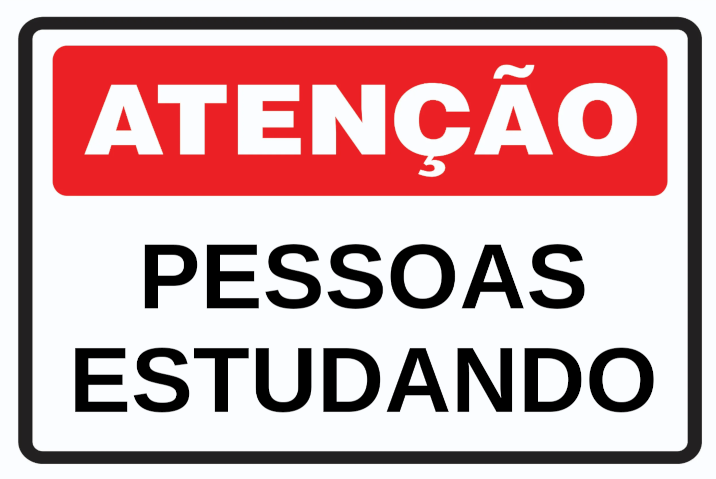
\includegraphics[scale=0.13]{imagens/fig-atencao-pessoas-estudando.png}
			
			%			\item \glsfirst{exercicio_014}: \glsdesc{exercicio_014}
			
		\end{itemize}
	}\par
	\vspace{1em}
	
	
	
\end{frame}








\begin{frame}[t]{Interface de classe}
	
	\fontsize{14pt}{15}\selectfont{
		
		Uma interface define um conjunto de métodos que uma classe deve implementar. Ela atua como um contrato.
		
	}\par
	\vspace{1em}
	
	\fontsize{12pt}{15}\selectfont{
		\begin{itemize}%[<+->] 
			
			\item Em Python, não há uma palavra-chave específica para definir \textbf{interfaces}, mas podemos usar \textbf{classes abstratas} para criar \textbf{interfaces}.
			
		\end{itemize}
	}\par
	\vspace{1em}
	
\end{frame}


\begin{frame}[t]{Classes Abstratas}
	
	\fontsize{14pt}{15}\selectfont{
		
		Uma classe abstrata é uma classe que não pode ser instanciada diretamente. Ela serve como um modelo para outras classes.
		
	}\par
	\vspace{1em}
	
	\fontsize{12pt}{15}\selectfont{
		\begin{itemize}%[<+->] 
			
			\item Podemos criar uma classe abstrata com o \textbf{módulo abc} (Abstract Base Classes) em Python.
			
		\end{itemize}
	}\par
	\vspace{1em}
	
	\url{https://docs.python.org/pt-br/3/library/abc.html}
	
\end{frame}


\begin{frame}[t]{Interface com Classes Abstratas - Caso com abc}
	\vspace{-0.75em}
%	\lstinputlisting[style=CBruno,caption=Classe Produto Abstrata]{outros/codigos/python/exemplos-de-aulas/src/codigo_012_classe_produto_abstrato.py}
	
	\centering
	\makebox[\linewidth][c]{
		\begin{minipage}{0.95\textwidth}
			\inputminted[fontsize={\fontsize{6}{7}\selectfont}]{python}{outros/codigos/python/exemplos-de-aulas/src/codigo_012_classe_produto_abstrato.py}
		\end{minipage}
	}
	\fontsize{7pt}{6}\selectfont{
		Classe Produto Abstrata - codigo\_012\_classe\_produto\_abstrato.py
	}\par
	
	
	\vspace{0.25em}
	\fontsize{9pt}{10}\selectfont{
		*obs: \textbf{pass} é usada como um espaço reservado quando o código é necessário, mas nenhuma ação específica é exigida. Use \textbf{pass} como um espaço reservado para posteriormente implementação.
	}\par
	
\end{frame}

\begin{frame}[t]{Interface com Classes Abstratas - Caso com abc}
	
	\vspace{-0.5em}
	
%	\lstinputlisting[style=CBruno,caption=Classe Produto Abstrato]{outros/codigos/python/exemplos-de-aulas/src/codigo_012_classe_produto_concreto.py}
	\centering
	\makebox[\linewidth][c]{
		\begin{minipage}{0.95\textwidth}
			\inputminted[fontsize={\fontsize{6}{7}\selectfont}]{python}{outros/codigos/python/exemplos-de-aulas/src/codigo_012_classe_produto_concreto.py}
		\end{minipage}
	}
	\fontsize{7pt}{6}\selectfont{
		Classe Produto Abstrata - codigo\_012\_classe\_produto\_concreto.py
	}\par
	
\end{frame}


\begin{frame}[t]{Pytest}
	
%	\vspace{1em}
%	\lstinputlisting[style=CBruno,caption=Cobertura de testes da classe Produto Concreto]{outros/codigos/python/exemplos-de-aulas/tests/test_codigo_012_classe_produto_concreto.py}

	\centering
	\makebox[\linewidth][c]{
		\begin{minipage}{0.95\textwidth}
			\inputminted[baselinestretch=1.15,fontsize={\fontsize{9}{9}\selectfont}]{python}{outros/codigos/python/exemplos-de-aulas/tests/test_codigo_012_classe_produto_concreto.py}
		\end{minipage}
	}
	\fontsize{7pt}{6}\selectfont{
		Cobertura de testes da classe Produto Concreto - test\_codigo\_012\_classe\_produto\_concreto.py
	}\par

\end{frame}


\begin{frame}[t]{Testes Unitários}
	
	
	\vspace{1em}
	\centering
	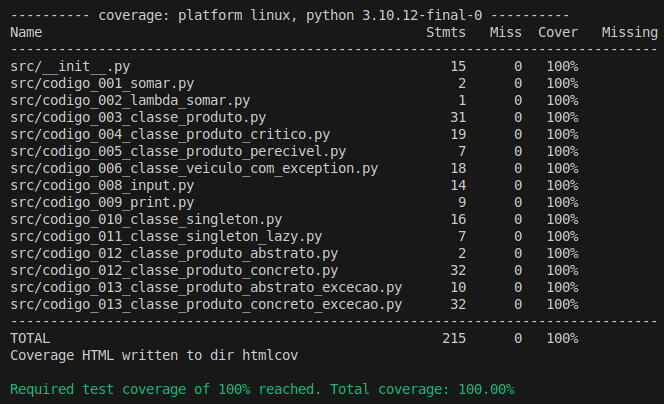
\includegraphics[scale=0.4]{imagens/fig-result-test-produto-concreto.png}
	
	\vspace{0.25em}
	\fontsize{9pt}{10}\selectfont{
		*obs: \textit{pytest --maxfail=1  --cov-fail-under=100 --disable-warnings --cov=./src --cov-report=html --cov-report=term-missing}
	}\par
	
\end{frame}






\begin{frame}[t]{Interface com Classes Abstratas - Caso com Exceção}
	
%	\lstinputlisting[style=CBruno,caption=Classe Produto Abstrato Excecao]{outros/codigos/python/exemplos-de-aulas/src/codigo_013_classe_produto_abstrato_excecao.py}
	
	\centering
	\makebox[\linewidth][c]{
		\begin{minipage}{0.95\textwidth}
			\inputminted[baselinestretch=1,fontsize={\fontsize{8}{8}\selectfont}]{python}{outros/codigos/python/exemplos-de-aulas/src/codigo_013_classe_produto_abstrato_excecao.py}
		\end{minipage}
	}
	\fontsize{7pt}{6}\selectfont{
		Classe Produto Abstrato Exceção - codigo\_013\_classe\_produto\_abstrato\_excecao.py
	}\par
	
	
\end{frame}

\begin{frame}[t]{Interface com Classes Abstratas - Caso com Exceção}
	\vspace{-0.5em}
%	\lstinputlisting[style=CBruno,caption=Classe Produto Concreto Excecao]{outros/codigos/python/exemplos-de-aulas/src/codigo_013_classe_produto_concreto_excecao.py}
	\centering
	\makebox[\linewidth][c]{
		\begin{minipage}{0.95\textwidth}
			\inputminted[fontsize={\fontsize{6}{6}\selectfont}]{python}{outros/codigos/python/exemplos-de-aulas/src/codigo_013_classe_produto_concreto_excecao.py}
		\end{minipage}
	}
	\fontsize{7pt}{6}\selectfont{
		Classe Produto Concreto Exceção - codigo\_013\_classe\_produto\_abstrato\_excecao.py
	}\par
\end{frame}


\begin{frame}[t]{Testes Unitários}
	
%	\vspace{-1em}
%	\lstinputlisting[style=CBruno,caption=Cobertura de testes da classe Produto Concreto Exceção]{outros/codigos/python/exemplos-de-aulas/tests/test_codigo_013_classe_produto_concreto_excecao.py}
	
	\centering
	\makebox[\linewidth][c]{
		\begin{minipage}{0.95\textwidth}
			\inputminted[baselinestretch=1,fontsize={\fontsize{9}{8}\selectfont}]{python}{outros/codigos/python/exemplos-de-aulas/tests/test_codigo_013_classe_produto_concreto_excecao.py}
		\end{minipage}
	}
	\fontsize{7pt}{6}\selectfont{
		Cobertura de testes da classe Produto Concreto Exceção - test\_codigo\_013\_classe\_produto\_concreto\_excecao.py
	}\par
	
\end{frame}









